% Preamble
% --------
\documentclass[12pt]{article}

\newcommand{\codename}[0]{\texttt{apex-sim}~}

% Packages
% --------
\usepackage{blindtext} %for boilerplate text (\blindtext)
\usepackage{geometry} %for paper dimensions and margins
\usepackage{graphicx} % for including graphics
\usepackage{hyperref} % for hyperlink support

% Page Setup
% ----------
\geometry{letterpaper, margin=1in}

% Title content and formatting
% ----------------------------
\title{Apex Instruction Set Architecture Simulator (\texttt{apex-sim}) \\ Phase 1 Documentation}
\author{Matthew Cole \\ \texttt{mcole8@binghamton.edu}
\and
Brian Gracin \\ 
	\texttt{bgracin1@binghamton.edu}}
\date{19 November 2016}

\begin{document}
% Emit title content
% ------------------
\pagenumbering{gobble}
\maketitle
\tableofcontents
\listoffigures
\newpage
\pagenumbering{arabic}

%---------------

\section{Design}
\codename is a simulator for the \textit{Architecture Pipeline EXample} (APEX) Instruction Set Architecture (ISA).
\codename consists of the following components:
\begin{itemize}
  \item \texttt{main.cpp} contains the driver program. The driver program provides file input for instructions, user interface operations, and maintaining persistent simulator state. This component is discussed in section \ref{sec:driver}.
  \item \texttt{code.cpp}, \texttt{data.cpp}, \texttt{registers.cpp}, \texttt{cpu.cpp}, and \texttt{stage.cpp} provide the objects modeling components of the pipeline. These components are discussed in section \ref{sec:classes}.
  \item \texttt{simulate.cpp} provides the functions that allow the CPU to simulate working on each of its stages, inter-stage communication through advancement, stalls for basic inter-stage interlocks, and forwarding. These implementation details are described in section \ref{sec:implementation}.
\end{itemize}
Figure \ref{fig:overview} shows class interactions and data flow between each of the stages and support classes.
Finally, we opensource our work under the MIT license through a GitHub repository located at \url{https://github.com/colematt/apex-sim}. We discuss our team's work log in section \ref{sec:production}.

\begin{figure}
  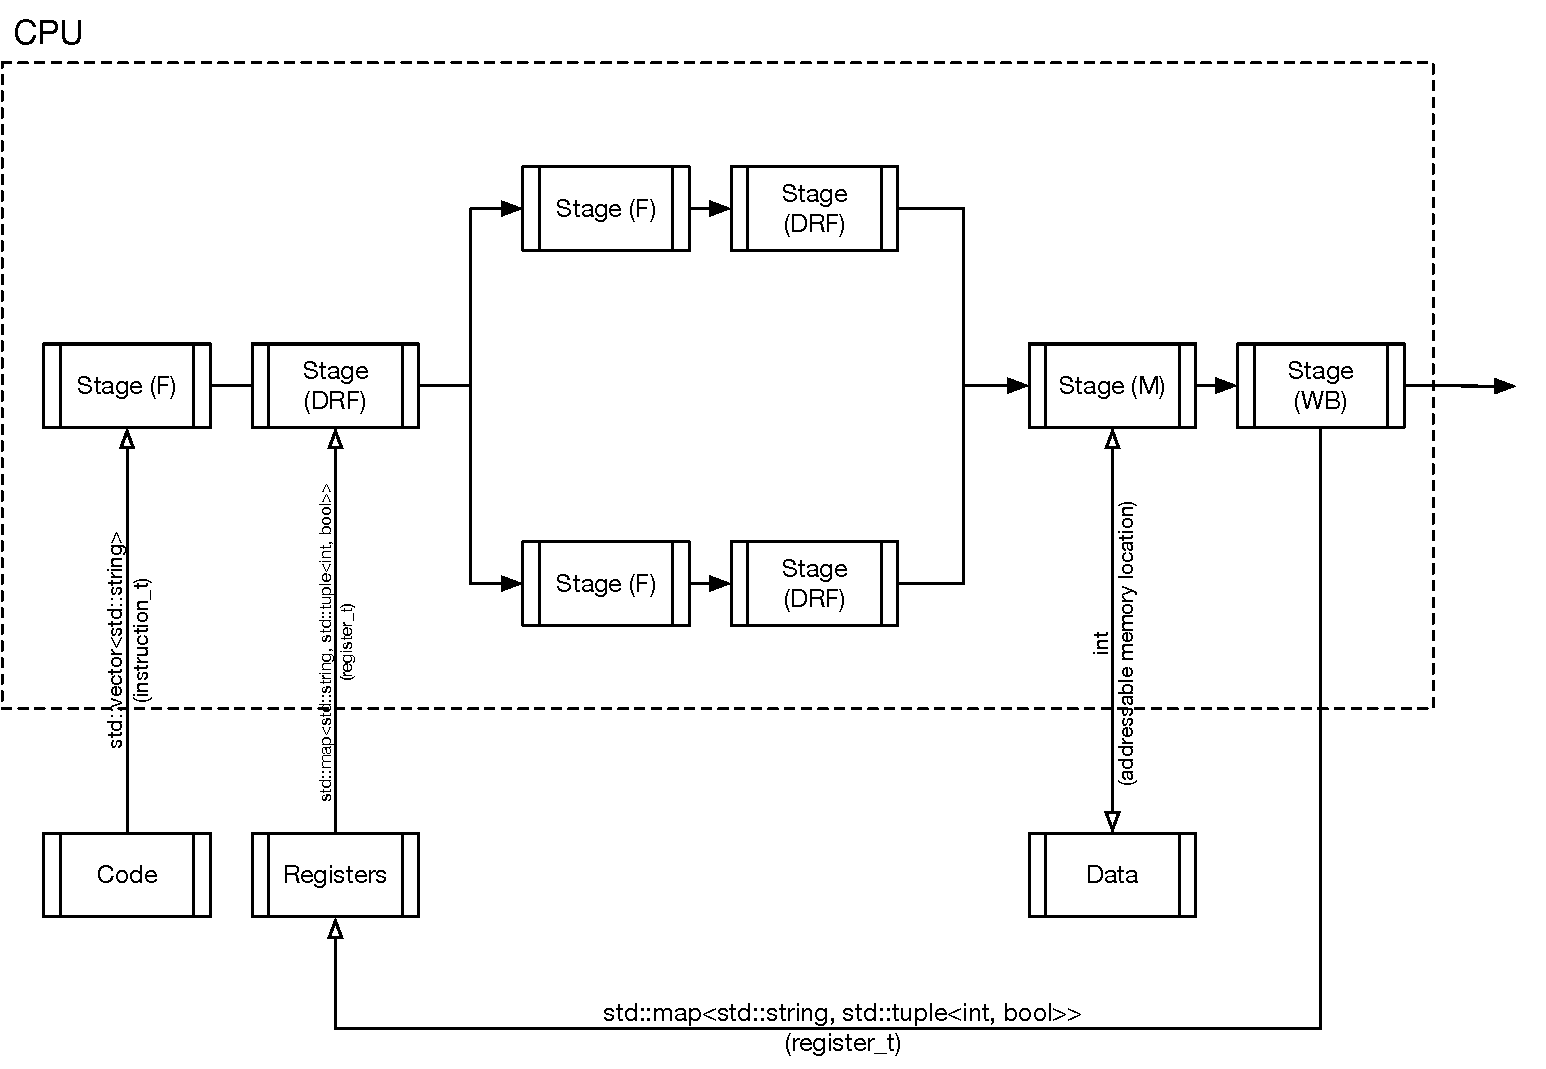
\includegraphics[width=\linewidth]{./figs/apex-sim-overview.pdf}
  \caption{APEX pipeline and class interactions.}
  \label{fig:overview}
\end{figure}

\subsection{Driver Program}
\label{sec:driver}
The \codename entry point file is \texttt{main.cpp}. Besides maintaining simulator state variables for the current cycle, program counter and instructions filename, this program shepherds execution through the lifecycle of the program and provides a user interface for interacting with the simulator. The functionality of the driver program is as follows:
\begin{enumerate}
  \item Verify sanity of command line inputs (lines 107-116).
  \item Instantiate class instances for the simulator (lines 119-122).
  \item Perform the initialization of each pipeline stage (line 125).
  \item Prepare and begin the simulator user interface's operations (lines 128-134).
  \item Parse user interface inputs and delegate actions to interface helper functions (lines 134-161).
\end{enumerate}

\texttt{main.cpp} also provides helper functions which delegate work down to class instances. These functions are:
\begin{itemize}
  \item \texttt{help()} displays the user interface keyboard shortcuts. It's invoked at startup, on request from the user, and whenever the user provides an input which is not recognized.
  \item \texttt{initialize()} resets the simulator state, and invokes the class instances' own \texttt{\textit{classname}.initialize()} functions which reset the instances' internal state.
  \item \texttt{display()} displays the simulator internal state variables as well as delegated calls to each class' \texttt{\textit{classname}.display()} function.
  \item \texttt{quit()} gracefully halts the simulator and triggers a final call to \texttt{display()}.
  \item \texttt{simulate()} is the most important of the helper functions. It is responsible for controlling simulation of the \texttt{CPU.simulate()} function for a given number of cycles, and allowing the CPU class to communicate that it has encountered an error, reached EOF of a code file without a HALT instruction, or has processed a HALT instruction through the pipeline.
\end{itemize}

\subsection{Classes}
\label{sec:classes}
\codename models each major component of the APEX system as a standalone class. These classes are discussed in the following sections.

\subsubsection{Code}
The code class performs two roles. 
First, during its construction, it reads a text file into a vector container. This decision was made because random access into a vector is trivial, while random access into a text file whose lines are not a constant length (as in the APEX ISA) is extremely challenging. 
Second, those instructions are tokenized by first separating the opcode from its operands by searching for a whitespace character from the beginning of the string, then separating the remainder of the string on commas. 

The final result is that the Code class allows us to receive a pre-parsed instruction simply by specifying a program counter value corresponding to a line in the input text file. 
As stated in the specification, with a 0-based index, the $k^{th}$ line is the instruction corresponding to program counter value $4000 + 4k$. 
Instructions can be easily read into the Fetch stage using the \texttt{std::vector<std::string> Code::getInstr(int addr)} member function.

Unlike the other classes, Code does not provide a means of modifying the values it contains. This is because a code segment is ordinarily not writeable by programs once execution has begun (with exceptions such as Just-In-Time code). \codename models this behavior by prohibiting modifying a Code object after construction. Its contents can be found by reading the source code input text file; accordingly, \codename Code objects do not have a \texttt{display()} method, unlike many of the other component classes.

\subsubsection{Data}
The Data class is similar to the code because it provides the ability for the APEX pipeline to interact with main memory for long-term storage.
(Note: the APEX pipeline does not have a concept of cache levels; the pipeline writes and reads directly from memory). 
As a result, Data instances provide an API consisting of two functions: \texttt{int Data::readMem(int addr)} and \texttt{void Data::writeMem(int addr, int value)}. 
These function as basic class accessor and mutator respectively.
Because APEX has no concept of memory-to-memory operations, only two Data manipulation instructions exist: LOAD and STORE.
\codename only uses the Data accessor and mutator functions in the Memory (MEM) stage.

Underneath this exposed interface, the Data class uses a vector container consisting of 4000 integer values. 
Although 4000 integers exist, in the APEX specification, only 4-byte aligned values are addressable. 
Therefore, the unaligned addresses remain unused, and the aligned values of the vector are limited in size to 4 bytes wide (half the width of a 64-bit system integer primitive). This was done for developer convenience, and it is transparent to the user in practice.

\subsubsection{Registers}
\codename models a register file containing infinite virtual read and write ports using the Registers class.
Each register in the register file has three components: a key \-- a string containing the name of the register, and a two-tuple value \-- an integer containing the \textit{value} of the register and a bool containing the \textit{validity}. 
The validity of the register is used for simple interlocking as a means of managing flow dependencies across a register.
This (and the process of stalling) is further discussed in section \ref{sec:stalls}.

A Registers instance contains sixteen general purpose registers labelled with the strings "R0" through "R15". 
There are also two special purpose registers "X" and "Z".
Strictly speaking, we do not perform any checking for source code which attempts to use these registers.
However, from the Specification, the "X" register is understood to be used to store the most recent return address (i.e. PC + 4) for BAL calls, and the "Z" register is set only as the last arithmetic value calculated in the second ALU (ALU2) stage (i.e. for BZ/BNZ instructions).
These special purpose registers are not to be employed by an APEX programmer for general use.
Forwarding destination set general purpose registers and the "X" and "Z" registers is discussed in section \ref{sec:forwarding}.

The Registers class provides two accessors and one mutator. There are two accessors, one for each of value and validity of a given register key. 
The reason for only having one mutator is to require an update of validity each time a value is set in the Write Back (WB) phase.
Underneath this exposed interface, the Registers class is an associative map mapping a string to a two-tuple of integer and bool primitives. 
This design decision allows strings representing register names in the assembly code to randomly access values without further translating the string each time to extract the register number, and allows registers to be named without any indication of ordering (i.e. "X" or "Z"). 
This would have been substantially more difficult with a vector accessed by offset index.

\subsubsection{CPU and Stages}
The CPU class in \codename contains a total of eight instances Stage classes, as described in the Specification. The CPU class therefore serves two purposes. 
First, it provides a \texttt{simulate()} function which causes work to occur in each stage. 
Second \texttt{simulate()} allows communication between classes for advancing the in-flight instructions and for forwarding.  
CPU's delegation and inter-class communication is similar to a Visitor design pattern without abstract class implementations. 
This design decision was made solely for expediency. 
We acknowledge that a more robust design would use a combination of a Visitor design pattern with threaded instances of each class to simulate simultaneous execution of each stage's work (as opposed to our reverse-order shepherding model, described in section \ref{sec:implementation}).

CPU class also provides delegation functions which call \texttt{initialize()}, \texttt{display()} on its Stage instances on behalf of \texttt{main.cpp} during simulator execution.

%-----------------------
\section{Implementation}
\label{sec:implementation}
In this section, we will discuss three key aspects of our simulator's execution: the stage-wise reverse-ordered execution, simple interlocking and stalls, and register value forwarding.

\subsection{Stage-wise Reverse Order Execution}

\subsection{Stalls}
\label{sec:stalls}

\subsection{Forwarding}
\label{sec:forwarding}
\codename uses data forwarding as a means of reducing delays caused by flow dependencies.
The forwarding paths used by \codename are shown in figure \ref{fig:forwarding}, and a description of each follows:

\subsubsection{LOAD instruction in Memory stage}

\subsubsection{Arithmetic or MOVC instructions in ALU2 stage}

\subsubsection{BAL instructions in Branch, Delay, or Memory stage}

\begin{figure}
  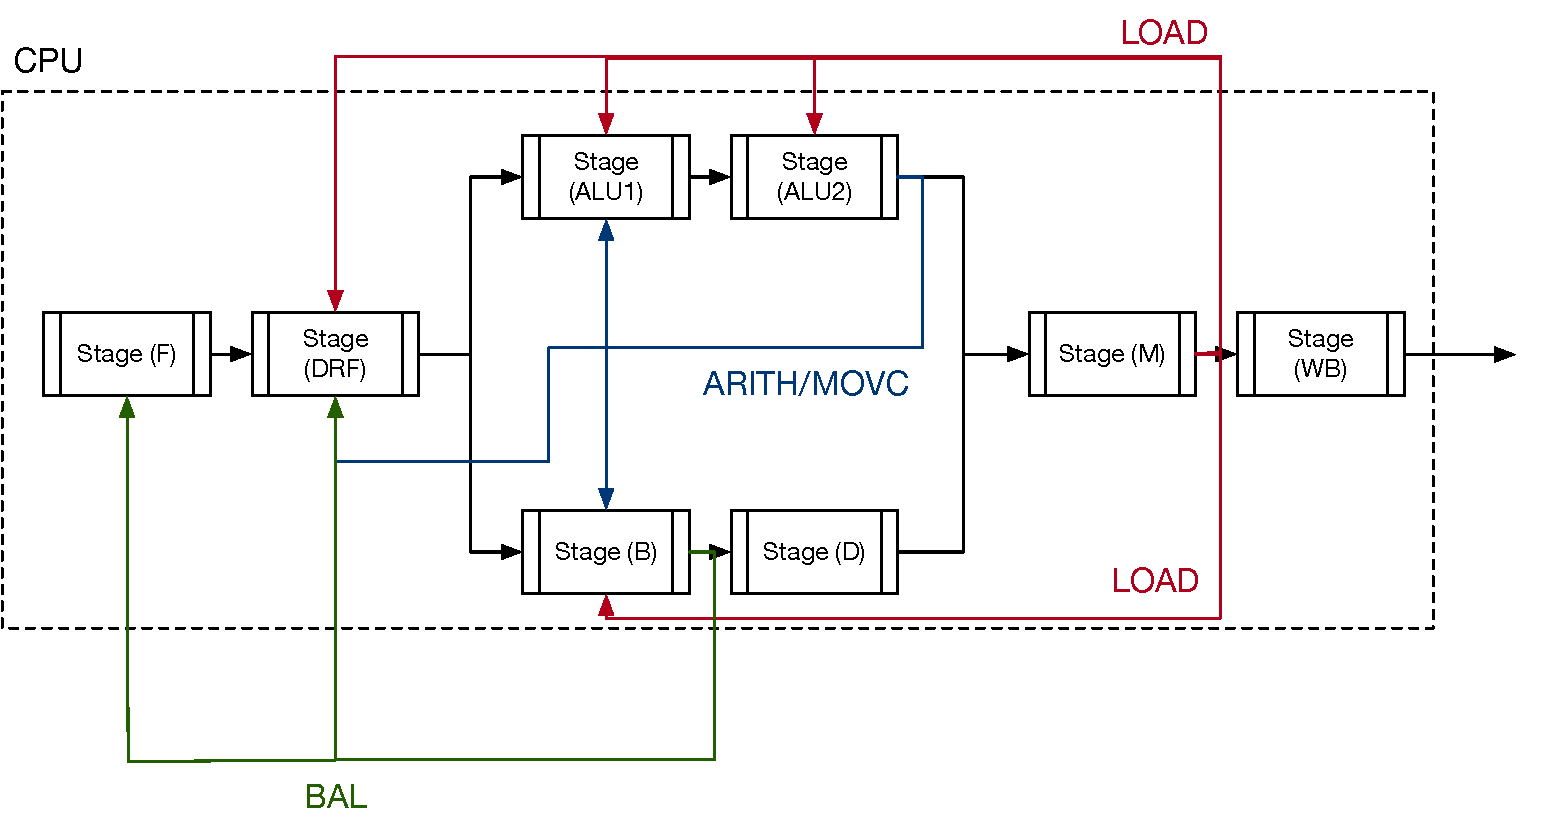
\includegraphics[width=\linewidth]{./figs/apex-sim-forwarding.pdf}
  \caption{APEX pipeline forwarding paths.}
  \label{fig:forwarding}
\end{figure}

%-------------------
\section{Production}
\label{sec:production}

\end{document}


